\documentclass[aspectratio=169]{beamer}

\usepackage{mathtools}
\usepackage{qrcode}
\usepackage{tikz}

% A small note pinned to the same spot at the bottom of every slide.
\newcommand{\slidenote}[1]{%
  \begin{tikzpicture}[remember picture, overlay]
    \node[anchor=south west, inner sep=0pt, text width=0.9\paperwidth,
          font=\footnotesize]
      at ([xshift=0.05\paperwidth, yshift=0.06\paperheight]current page.south west)
      {#1};
  \end{tikzpicture}%
}

\usetheme{default}
\setbeamertemplate{navigation symbols}{}

\title{Collaborative Filtering for Movie Recommendations}
\author{Saku Suuriniemi}
\institute{Reaktor}
\date{\today}

\begin{document}

\begin{frame}
  \titlepage
\end{frame}

\begin{frame}{The question}
  \begin{center}
    \large How can a short list of movies you like lead to useful recommendations?
  \end{center}

  \begin{itemize}
    \item Learn movie-to-movie relationships from synthetic viewer likes.
    \item Use a new viewer's favorites to rank unseen movies in IMDb's Top 1000.
    \item Compare L2 and L1 regularization, then try recommendations in Streamlit.
  \end{itemize}

  \slidenote{Synthetic preferences make this a teaching example, not evidence
  of real-world recommendation quality.}
\end{frame}

\begin{frame}{Starting from your favorites}
  \begin{itemize}
    \item \textbf{Catalog:} IMDb's Top 1000 movies
    \item \textbf{Your input:} a few of your favorite movies
    \item \textbf{Collaborative filtering:} learn from other viewers' preferences
  \end{itemize}

  \begin{itemize}
    \item Fix an order for the 1,000 movies.
    \item Encode your favorites as a sparse vector, $v \in \{0,1\}^{1000}$.
    \item $v_i = 1$: movie $i$ is a favorite; $v_i = 0$ otherwise.
  \end{itemize}

  \slidenote{Zero means unknown, not disliked.}
\end{frame}

\begin{frame}{What to do with your sparse vector?}
  \begin{itemize}
    \item Set up a simple linear model with a matrix $X$ of movie-to-movie relationships.
    \item Multiply your sparse vector by this matrix to get scores for all movies.
    \item Rank the movies by these scores to generate recommendations.
  \end{itemize}

  \begin{center}
    Where to get this matrix?
  \end{center}

\end{frame}


\begin{frame}{Where do the likes come from? (Synthetic!)}
  \begin{itemize}
    \item 50,000 fake viewers, each with 1--3 favorite genres, a few directors and actors.
    \item Each viewer likes about 20 movies: 90\% chosen by taste match, 10\% by IMDb popularity.
  \end{itemize}

  \begin{block}{Consequence}
    The model can only learn what is in the data: here, shared genres, directors and actors.
    Odd results (Toy Story $\Rightarrow$ Airplane!, both comedies) come from the fake viewers, not the method.
  \end{block}
\end{frame}

\begin{frame}{Learning movie-to-movie relationships}
  \begin{itemize}
    \item Collect one sparse like-vector per viewer.
    \item Stack them as columns of $H \in \{0,1\}^{M \times N}$.
  \end{itemize}

  \[
    H \approx XH,
    \qquad X \in \mathbb{R}^{M \times M}
  \]

  \begin{itemize}
    \item $X = I$ copies the input likes: a trivial perfect reconstruction.
    \item Forbid self-prediction: $\operatorname{diag}(X) = 0$.
  \end{itemize}

  \slidenote{$M$: movies \qquad $N$: viewers}
\end{frame}

\begin{frame}{The optimization problem}
\[
\min_X \|H - XH\|_F^2
\qquad \operatorname{diag}(X) = 0
\]

\begin{itemize}
  \item First term: reconstruction error
  \item Constraint: no self-prediction
\end{itemize}

\vspace{1em}
\slidenote{The Frobenius norm measures the sum of squared differences between the predicted and actual likes.}
\end{frame}

\begin{frame}{Why keep movie connections in check?}
  \begin{itemize}
    \item For rarely liked movies, very strong coincidental connections can arise.
    \item Example: 4 of the 5 viewers who liked a rare movie also liked
      \emph{Totoro}. The connection is 0.8, based on just 4 people.
    \item A penalty $\lambda$ shrinks connections built on little evidence;
      well-supported ones barely change.
  \end{itemize}
\end{frame}

\begin{frame}{L2: penalise large connections}
  \[
    \min_X \quad \underbrace{\|H - XH\|_F^2}_{\text{difference in likes}}
    \; + \; \underbrace{\lambda\|X\|_F^2}_{\text{penalty for large connections}}
  \]
  \[
    \text{subject to} \quad \underbrace{X_{ii} = 0}_{\text{no self-prediction}}
  \]

  \vspace{1em}
  \begin{center}
    $\lambda$ sets the penalty; how to set it?
  \end{center}
\end{frame}

\begin{frame}{Choosing $\lambda$ with Recall@10}
  \begin{itemize}
    \item Fit one model per candidate $\lambda$, using the training viewers.
    \item For each validation viewer, show five likes and hide the rest.
    \item Recommend ten movies and count how many hidden likes they contain.
  \end{itemize}

  \[
    \mathrm{Recall@10} =
    \frac{\text{hidden likes in the top ten}}{\text{all hidden likes}}
  \]

  \begin{itemize}
    \item Pick the $\lambda$ with the highest average Recall@10.
  \end{itemize}
\end{frame}

\begin{frame}{Keep the test viewers out}
  \begin{itemize}
    \item \textbf{Training} viewers: fit the models.
    \item \textbf{Validation} viewers: choose $\lambda$.
    \item \textbf{Test} viewers: a final check only, after everything is decided.
  \end{itemize}

  \vspace{1em}
  Why? If the test viewers help choose $\lambda$, the test score is too
  optimistic, and you only find out in production.
\end{frame}

\begin{frame}{Is 0.026 good?}
  \begin{center}
    \begin{tabular}{lccc}
      Recommender & \textbf{Validation} & \textbf{Test} & vs.\ random \\
      \hline
      Random 10 movies & $\approx 0.010$ & $\approx 0.010$ & $1\times$ \\
      Popularity (same list for everyone) & $0.019$ & $0.018$ & $1.9\times$ \\
      L1, $\lambda = 10$ & $0.023$ & $0.023$ & $2.3\times$ \\
      L2, $\lambda = 10{,}000$ & $0.026$ & $0.025$ & $2.6\times$ \\
      \hline
      Perfect model (knows true tastes) & $0.065$ & $0.066$ & $6.5\times$ \\
    \end{tabular}

    \footnotesize Recall@10. Test viewers were scored once, after $\lambda$ was chosen.
  \end{center}
\end{frame}

\begin{frame}{What the numbers mean}
  \begin{itemize}
    \item L2 finds about 35\% more hidden likes than popularity.
    \item At volume this is money: e.g.\ 10 million top-ten lists a day
      $\Rightarrow$ $\sim$35\% more successful recommendations, for one matrix solve.
    \item Even a perfect model that knows each viewer's true taste scores only 0.065:
      which 20 movies someone happened to like is largely luck.
  \end{itemize}
\end{frame}

\begin{frame}{The solution}
  \begin{itemize}
    \item This problem is a constrained least squares problem with an L2 regularization term.
    \item It has a closed-form solution for each $\lambda$ using standard linear algebra techniques.
  \end{itemize}

  \slidenote{Sketch of proof: build the unconstrained Lagrangian problem and differentiate to get a 1st degree problem.}
\end{frame}

\begin{frame}{Sparse solutions}
  \begin{itemize}
    \item L1 penalizes the sum of absolute connection strengths.
    \item Some connections become exactly zero, leaving a sparser model.
    \item Solve each movie's regression with scikit-learn's \texttt{Lasso}.
    \item Coordinate descent is iterative; unlike L2, there is no closed-form solution.
  \end{itemize}

  \[
    \min_X \|H - XH\|_F^2 + \lambda\|X\|_1
    \qquad \text{subject to} \quad X_{ii} = 0
  \]

  \slidenote{In the demo, L2 is trained live; L1 is precomputed because fitting it takes too long.}

\end{frame}

\begin{frame}[plain]
  \centering
  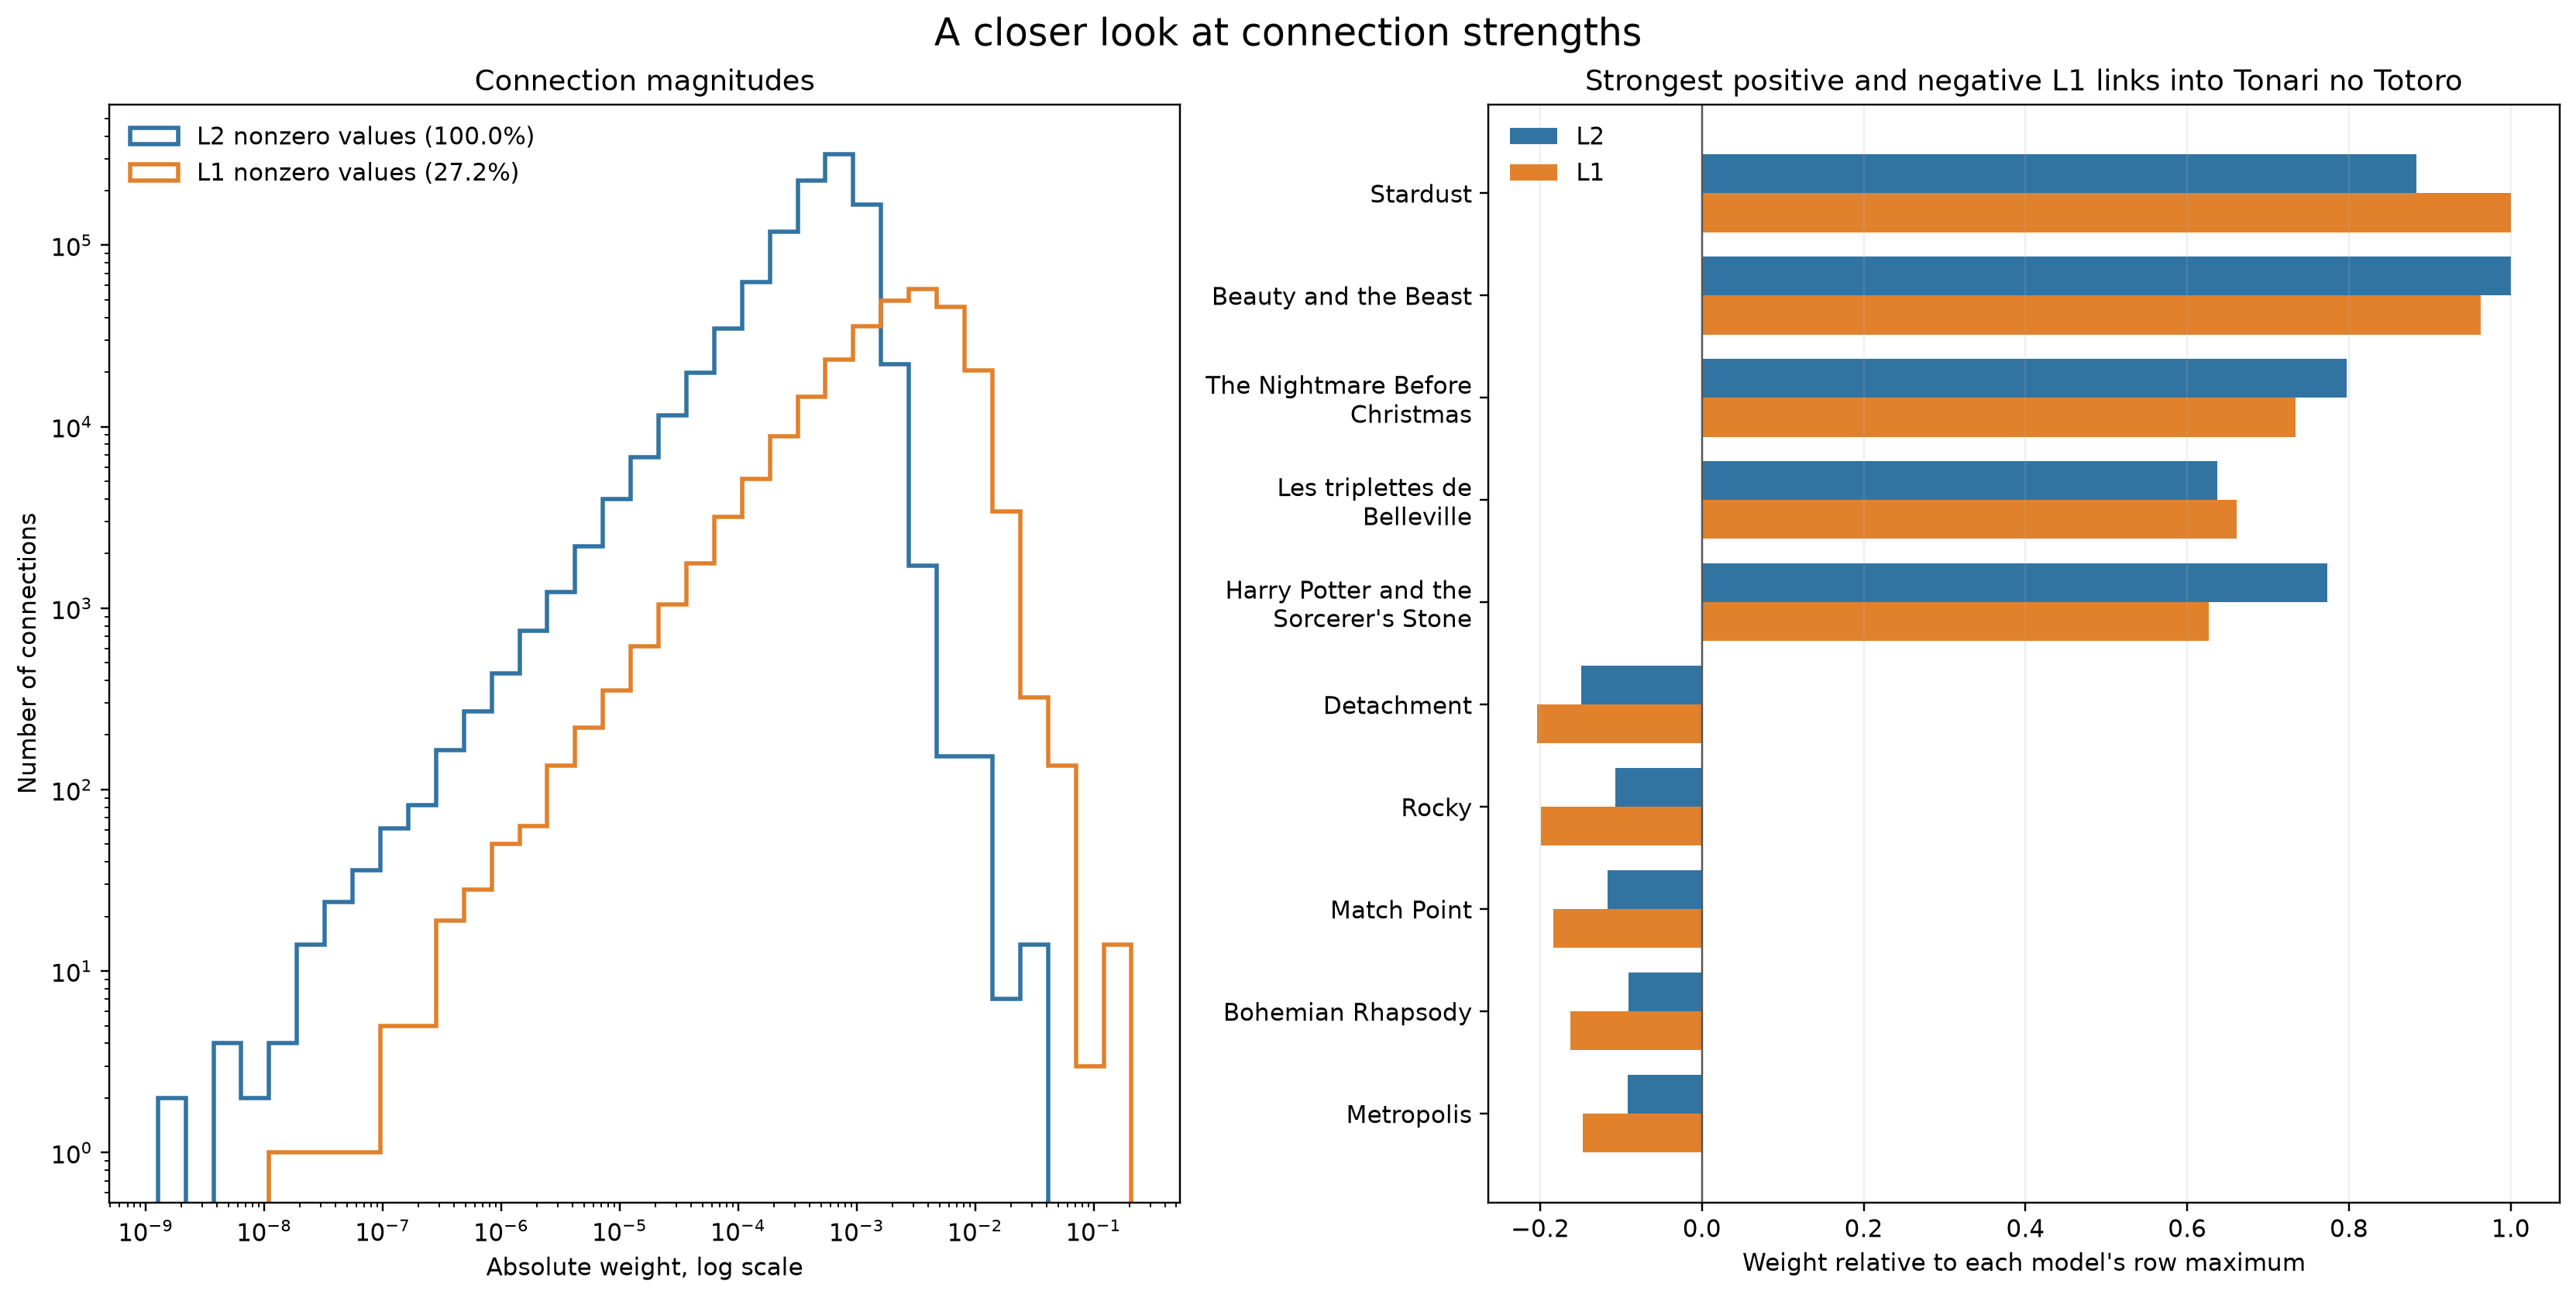
\includegraphics[
    width=0.96\textwidth,
    height=0.96\textheight,
    keepaspectratio
  ]{slides/assets/l1-l2-signed-links-full.png}
\end{frame}

\begin{frame}[plain]
  \centering
  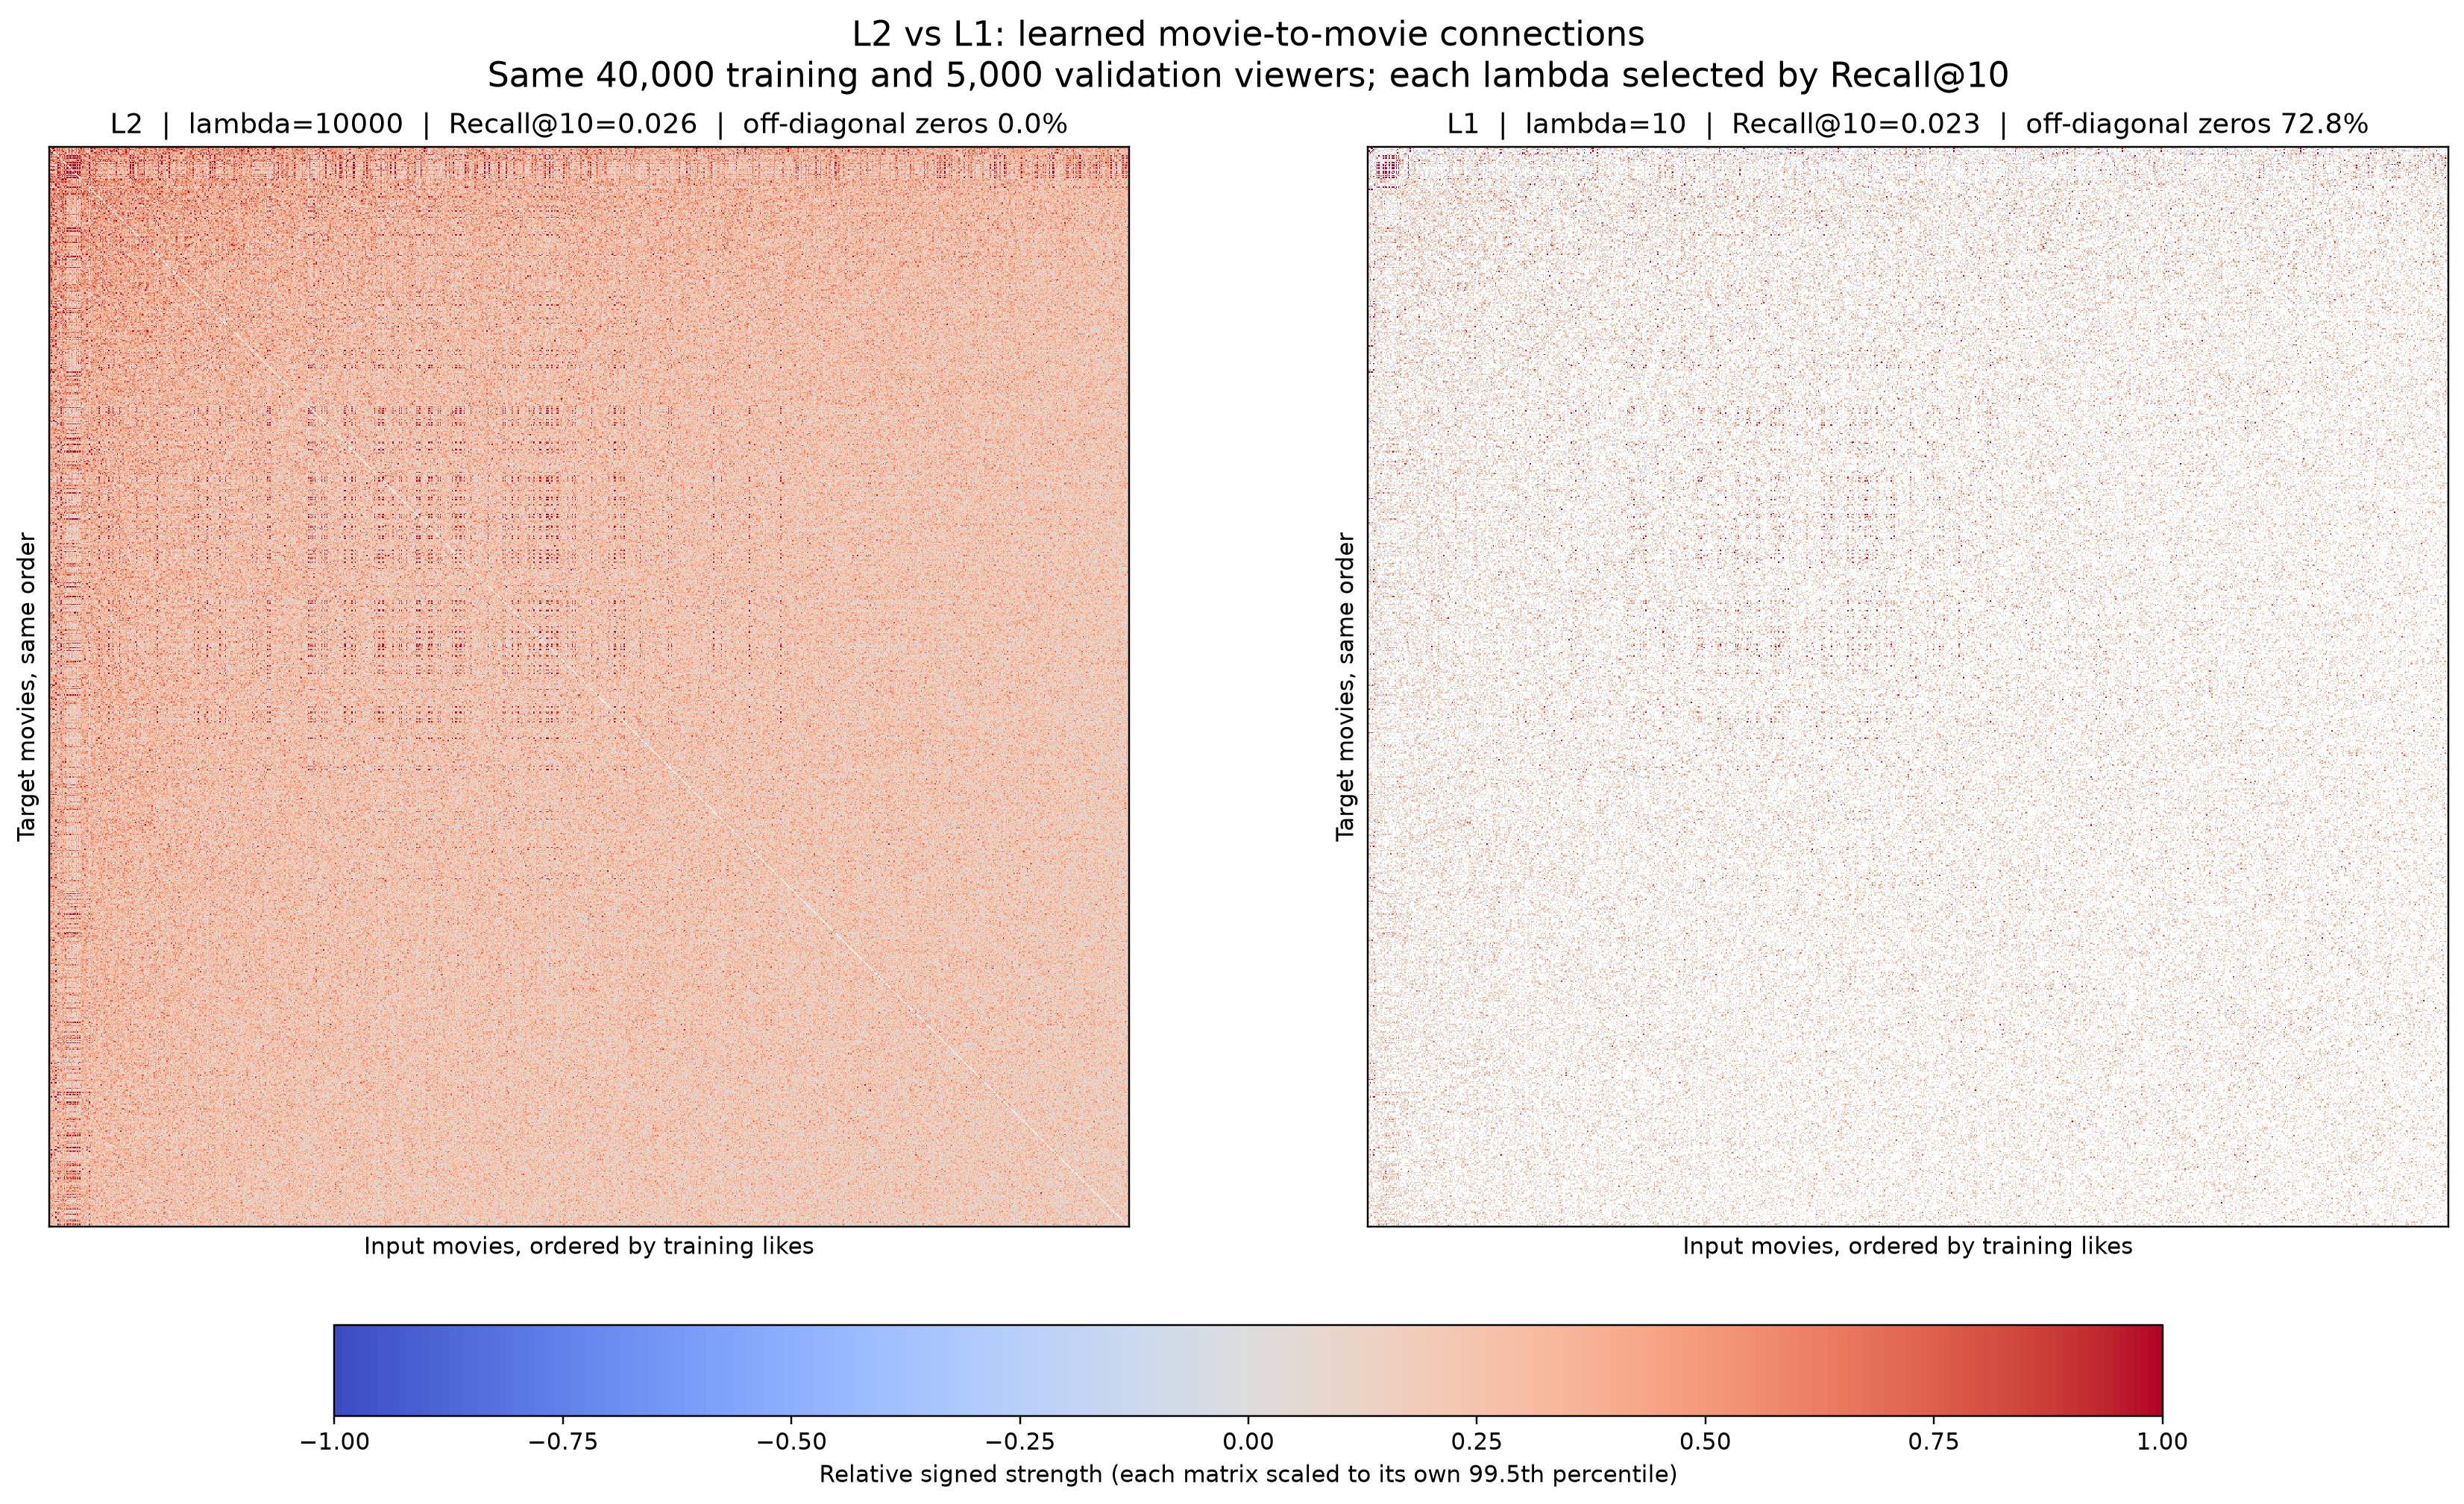
\includegraphics[
    width=0.96\textwidth,
    height=0.96\textheight,
    keepaspectratio
  ]{slides/assets/l1-l2-comparison-full.png}
\end{frame}

\begin{frame}{Summary}
  \begin{itemize}
    \item We formulated the movie recommendation problem as a constrained least squares problem.
    \item L2 regularization controls the magnitude of connections and has a closed-form solution.
    \item L1 regularization encourages sparsity but requires iterative optimization.
    \item Proper train-validation-test split is crucial for selecting the regularization parameter $\lambda$.
  \end{itemize}
\end{frame}

\begin{frame}[fragile]{Try it yourself}
  \begin{columns}[T]
    \begin{column}{0.62\textwidth}
      \footnotesize
\begin{semiverbatim}
git clone https://github.com/suurinie/\\
    movie-recommendation-demo-pyladies.git
cd movie-recommendation-demo-pyladies
uv sync --locked
uv run streamlit run src/movie_demo/app.py
\end{semiverbatim}

      \vspace{0.5em}
      No uv? Install it from \texttt{docs.astral.sh/uv}, or in a
      Python~3.12 virtual environment run \texttt{pip install -e .}
      and then \texttt{streamlit run src/movie\_demo/app.py}.
    \end{column}
    \begin{column}{0.34\textwidth}
      \centering
      \qrcode[height=3.8cm]{https://github.com/suurinie/movie-recommendation-demo-pyladies}

      \vspace{0.5em}
      \scriptsize github.com/suurinie/\\movie-recommendation-demo-pyladies
    \end{column}
  \end{columns}
\end{frame}

\end{document}